\documentclass[12pt]{scrartcl}

\usepackage[T1]{fontenc}
\usepackage[utf8]{inputenc}
\usepackage{amsmath}
\usepackage{amsfonts}
\usepackage{amssymb}
\usepackage{amsbsy}
\usepackage{graphicx}
\usepackage{float}
\usepackage{array}
\usepackage{booktabs}
\usepackage{multirow}
\usepackage{bm}
\usepackage{verbatim}
\usepackage[english]{babel}
\usepackage{color}
\usepackage{url}
\usepackage{fancybox}
\usepackage[stable]{footmisc}
\usepackage[format=plain,labelfont=bf]{caption}
\usepackage{fancyhdr}
\usepackage{natbib}
\usepackage{calc}
\usepackage{textcomp}
\usepackage[pdftex,pdfborder={0 0 0}]{hyperref}
\usepackage{pdfpages}
\usepackage{tikz}
\usetikzlibrary{shapes,backgrounds,fit,positioning,arrows,positioning,decorations.pathmorphing,decorations.pathreplacing,backgrounds}
\usepackage{accents}

\renewcommand*{\familydefault}{\sfdefault}

% Margins
\addtolength{\textheight}{1.0cm}
\addtolength{\oddsidemargin}{-0.5cm}
\addtolength{\evensidemargin}{-0.5cm}
\addtolength{\textwidth}{1.0cm}
\parindent=0em

% New math commands
\newcommand{\overbar}[1]{\mkern 1.5mu\overline{\mkern-1.5mu#1\mkern-1.5mu}\mkern 1.5mu}
\DeclareMathOperator{\diag}{diag}
\DeclareMathOperator{\Diag}{Diag}
\DeclareMathOperator{\tr}{tr}
\DeclareMathOperator{\var}{var}
\DeclareMathOperator{\Cov}{Cov}
\DeclareMathOperator{\Cor}{Cor}
\newcommand\independent{\protect\mathpalette{\protect\independenT}{\perp}}
\def\independenT#1#2{\mathrel{\setbox0\hbox{$#1#2$}%
\copy0\kern-\wd0\mkern4mu\box0}}

% Appropriate font for \mathcal{}
\DeclareSymbolFont{cmmathcal}{OMS}{cmsy}{m}{n}
\DeclareSymbolFontAlphabet{\mathcal}{cmmathcal}

% Set subscript and superscripts positions
\everymath{
\fontdimen13\textfont2=5pt
\fontdimen14\textfont2=5pt
\fontdimen15\textfont2=5pt
\fontdimen16\textfont2=5pt
\fontdimen17\textfont2=5pt
}

% Bibliography style
\setlength{\bibsep}{1pt}

% Part
\renewcommand\partheadstartvskip{\clearpage\null\vfil}
\renewcommand\partheadmidvskip{\par\nobreak\vskip 20pt\thispagestyle{empty}}
\renewcommand\partheadendvskip{\vfil\clearpage}
\renewcommand\raggedpart{\centering}

\begin{document}
\title{Shadow levels}
\author{Benjamin Ménétrier}
\date{Last update: \today}

\thispagestyle{empty}

\maketitle
\begin{center}
Copyright \copyright 2024: Meteorologisk Institutt
\end{center}

\tableofcontents

\section{Motivation}
For the convolution of 2D variables in correlation/localization implementations, orography can be very important (e.g. for snow over mountains). However, full 3D convolution is costly for two reasons: coefficients computation and normalization. It would be much more efficient to use existing horizontal convolution implementations (spectral, recursive filters, etc.) with an extra step to take orography into account.

\section{Theory}

\subsection{General framework}
The proposed solution is to surround a 3D horizontal convolution operator with shadow levels extension and reduction operators (mutually adjoint):
\begin{align}
\mathbf{C}_{2D} = \mathbf{F} \mathbf{C}_{3D} \mathbf{F}^\text{T}
\end{align}
where:
\begin{itemize}
\item $\mathbf{C}_{3D}$ is a 3D horizontal convolution operator,
\item $\mathbf{F}$ is the shadow levels reduction operator,
\item $\mathbf{F}^\text{T}$ is the shadow levels extension operator,
\item $\mathbf{C}_{2D}$ is the resulting 2D horizontal convolution operator.
\end{itemize}

\subsection{Shadow levels operators}
We define the $K$ shadow levels as vertical levels at constant height ${f_1, ..., f_K}$ in the orography vertical coordinate unit (e.g. meters). For each of the $n$ horizontal grid-points (listed with index $i$) and each shadow level $k$, a weight $w_k(i)$ is computed as:
\begin{align}
w_k(i) = \left\{ \begin{array}{cl}
c\left(\displaystyle \frac{f_k - z(i)}{r_v(i)}\right) & \text{if } f_k \ge z(i) \ \text{ [above surface]}\\
0 & \text{if } f_k < z(i) \ \text{ [below surface]}
\end{array} \right.
\end{align}
where:
\begin{itemize}
\item $c$ is a convolution function (e.g. Gaspari-Cohn 1999),
\item $z(i)$ is the local orography,
\item $r_v(i)$ is the local vertical convolution length-scale.
\end{itemize}
Weights are rescaled to ensure $\mathbf{C}_{2D}$ normalization:
\begin{align}
\overbar{w}_k(i) = \sqrt{\frac{w_k(i)}{\displaystyle \sum_{k'=1}^K w_{k'}(i)}}
\end{align}
and these normalized weights are the diagonal elements of weight matrices $\mathbf{W}^1, ..., \mathbf{W}^K$:
\begin{align}
\mathbf{W}^k = \left(\begin{array}{ccc}
\overbar{w}_k(1) & 0 & 0 \\
0 & \ddots & 0 \\
0 & 0 & \overbar{w}_k(n)
\end{array} \right)
\end{align}
The reduction operator $\mathbf{F}$ is given by:
\begin{align}
\mathbf{F} = \mathbf{R} \mathbf{W}
\end{align}
where $\mathbf{R}$ is a reduction matrix, i.e. a row of identity matrices:
\begin{align}
\mathbf{R} = \left(\begin{array}{ccc}
\mathbf{I} & \cdots & \mathbf{I}
\end{array}\right)
\end{align}
and $\mathbf{W}$ is the diagonal matrix of weight matrices:
\begin{align}
\mathbf{W} = \left(\begin{array}{ccc}
\mathbf{W}^1 & 0 & 0 \\
0 & \ddots & 0 \\
0 & 0 & \mathbf{W}^K
\end{array}\right)
\end{align}
Consistently, the extension operator is given by:
\begin{align}
\mathbf{F}^\text{T} = \mathbf{W} \mathbf{R}^\text{T}
\end{align}
since $\mathbf{W}$ is diagonal.\\
$  $\\
If we consider the horizontal field $T(i)$ and the 3D field $\hat{T}(i,k)$:
\begin{itemize}
\item the reduction operator $\mathbf{F}$ reduces $\hat{T}(i,k)$ into $T(i)$:
\begin{align}
T(i) = \sum_{k=1}^K \overbar{w}_k(i) \ \hat{T}(i,k)
\end{align}
\item the extension operator $\mathbf{F}^\text{T}$ extends $T(i)$ into $\hat{T}(i,k)$:
\begin{align}
\hat{T}(i,k) = \overbar{w}_k(i) \ T(i)
\end{align}
\end{itemize}

\subsection{Compactly supported functions}
For compactly supported functions (like Gaspari-Cohn 1999), and if shadow levels are too far apart, the orography $z(i)$ can be too far away from the surrounding shadow levels. For example:
\begin{itemize}
\item Shadow levels $f_1$ and $f_2$ are located at 0 and 100 m, respectively.
\item The convolution function $c$ has a compact support of radius 1.
\item The local orography is $z(i)$ = 45 m.
\item The local vertical convolution length-scale is $r_v(i)$ = 30 m.
\end{itemize}
In this case, the weights are:
\begin{align*}
\begin{array}{ccl}
f_1 < z(i)  & \Rightarrow & w_1(i) = 0 \\
f_2 \ge z(i) & \Rightarrow & w_2(i) = c\left(\displaystyle \frac{f_2 - z(i)}{r_v(i)}\right) = c\left(\frac{55}{30}\right) = 0
\end{array}
\end{align*}
As a consequence, it is not possible to compute the normalized weights $\overbar{w}$ and to define shadow levels operators. In the practical implementation, an exception should be thrown asking the user either to decrease the vertical distance between shadow levels $f_1$ and $f_2$, or to increase the value of $r_v(i)$.

\section{Illustration}

\subsection{Local orography}
With its steep orography, the Sognefjord region (western Norway) is well suited for testing the shadow levels method, as shown in Figure \ref{fig:orography}

\subsection{Shadow levels weights}
The normalized weights at different altitudes are displayed in Figure \ref{fig:weights}, showing a clear link to the remaining number of levels above surface:

\subsection{Dirac test at low altitude}
To clearly understand how the shadow levels work, we apply the convolution matrix $\mathbf{C}_{2D}$ on a Dirac vector $\boldsymbol{\delta}^j$:
\begin{align}
\delta_i^j =
\left\{ \begin{array}{ll}
1 & \text{ if } i = j \\
0 & \text{ elsewhere}
\end{array} \right.
\end{align}

In the first Dirac test, the impulse is located at a low altitude within the fjord, as shown in Figure \ref{fig:bottom_1-dirac_input}. Then, the extension operator $\mathbf{F}^\text{T}$ is applied on $\boldsymbol{\delta}^j$, as shown in Figure \ref{fig:bottom_2-split}. The horizontal 3D convolution operator $\mathbf{C}_{3D}$ is applied on $\mathbf{F}^\text{T} \boldsymbol{\delta}^j$ to give Figure \ref{fig:bottom_3-convolution}. The weight matrix $\mathbf{W}$ is applied in Figure \ref{fig:bottom_4-weighted_convolution} and the reduction matrix $\mathbf{R}$ in Figure \ref{fig:bottom_5-dirac_output}.\\

As expected, the resulting increment propagates horizontally following the fjord, but not at higher elevations. In a variational data assimilation system, an observation at the bottom of the fjord would not have any impact on the surrounding hills.

\subsection{Dirac test at high altitude}
The same test can be conducted with a Dirac impulse on a hill, Figures \ref{fig:top_1-dirac_input}, \ref{fig:top_2-split}, \ref{fig:top_3-convolution}, \ref{fig:top_4-weighted_convolution} and \ref{fig:top_5-dirac_output} show the same sequence. In that case, the increment is confined at high altitude. It propagates on surrounding hills, but not to the bottom of the fjord.

\subsection{Comparison with a full 3D convolution}
In Figure \ref{fig:small}, we compare the use of shadow levels with the reference of a full 3D convolution (using the BUMP library) at very high horizontal resolution. Both yield very similar results, the shadow levels methods being several orders of magnitude cheaper to run.

\clearpage

\section*{Figures}
In all the following figures, the red color map goes from 0 (white) to 1 (dark red).

\begin{figure}[!ht]
\centering
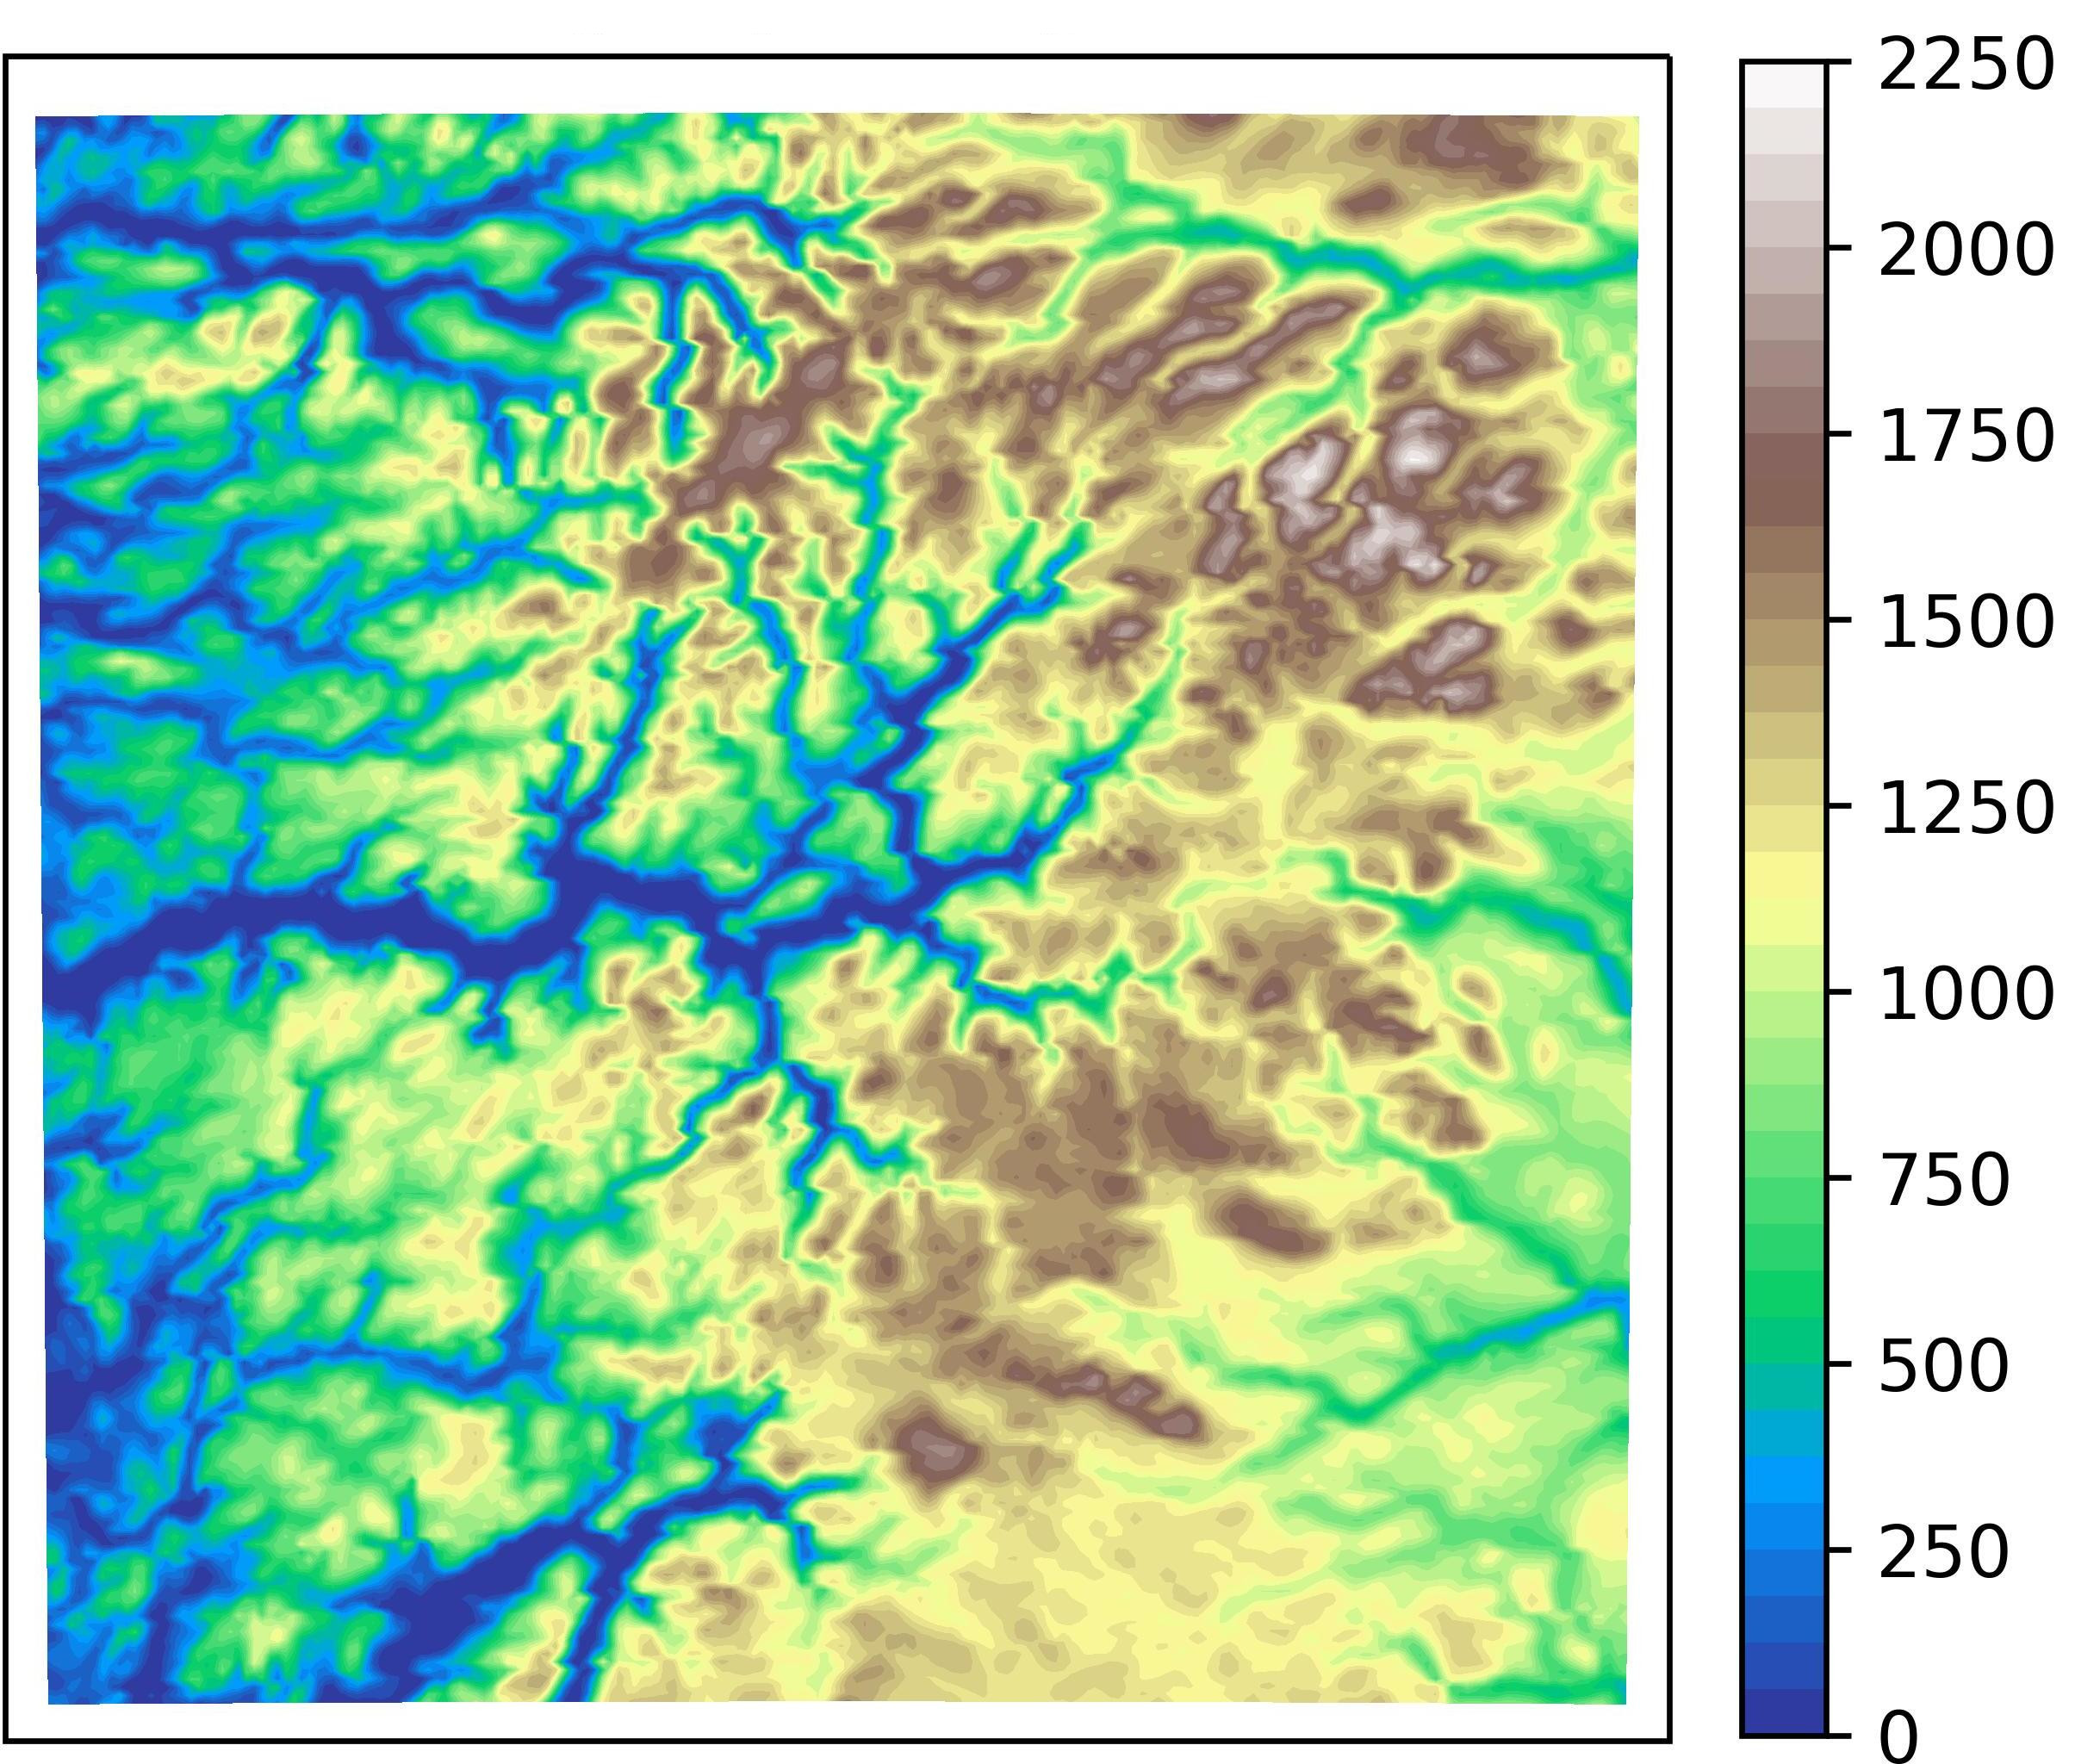
\includegraphics[width=0.5\textwidth]{orography.jpg}
\caption{Orography of the Sognefjord region (m)} \label{fig:orography}
\end{figure}

\begin{figure}[h!]
\centering
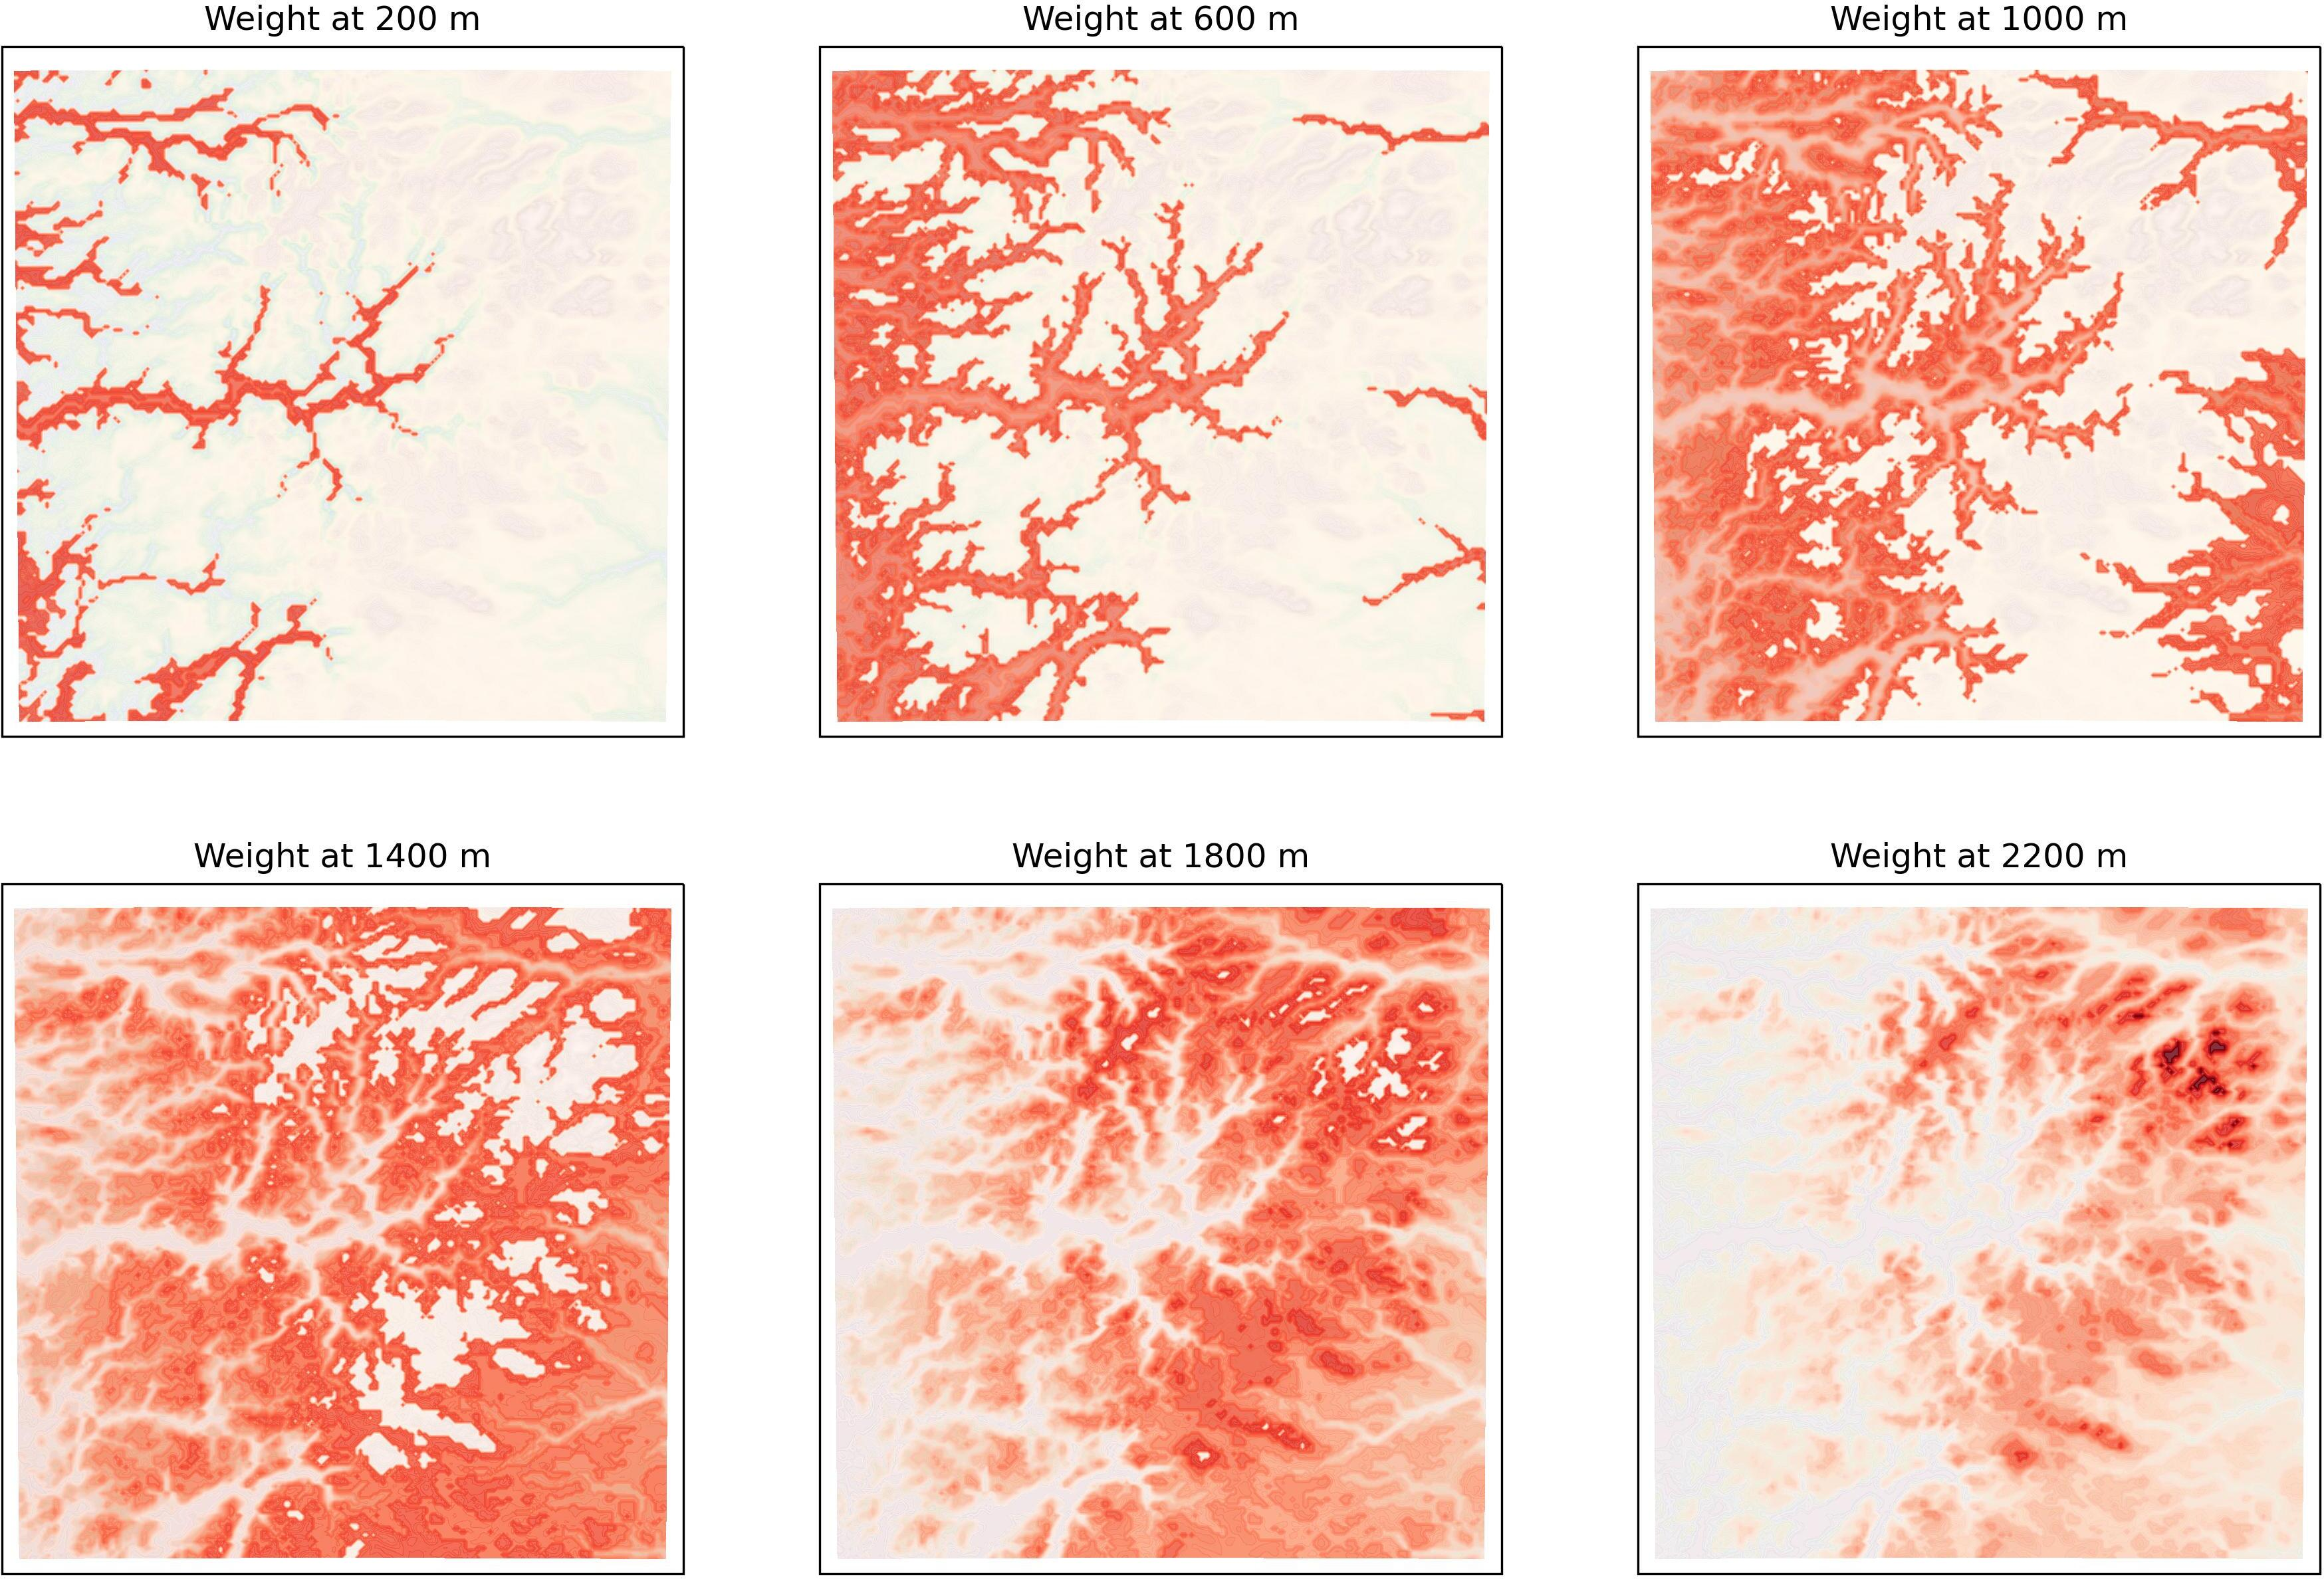
\includegraphics[width=\textwidth]{weights.jpg}
\caption{Normalized weights $\overbar{w}$ (values ranging from 0 to 1)} \label{fig:weights}
\end{figure}

\begin{figure}[h!]
\centering
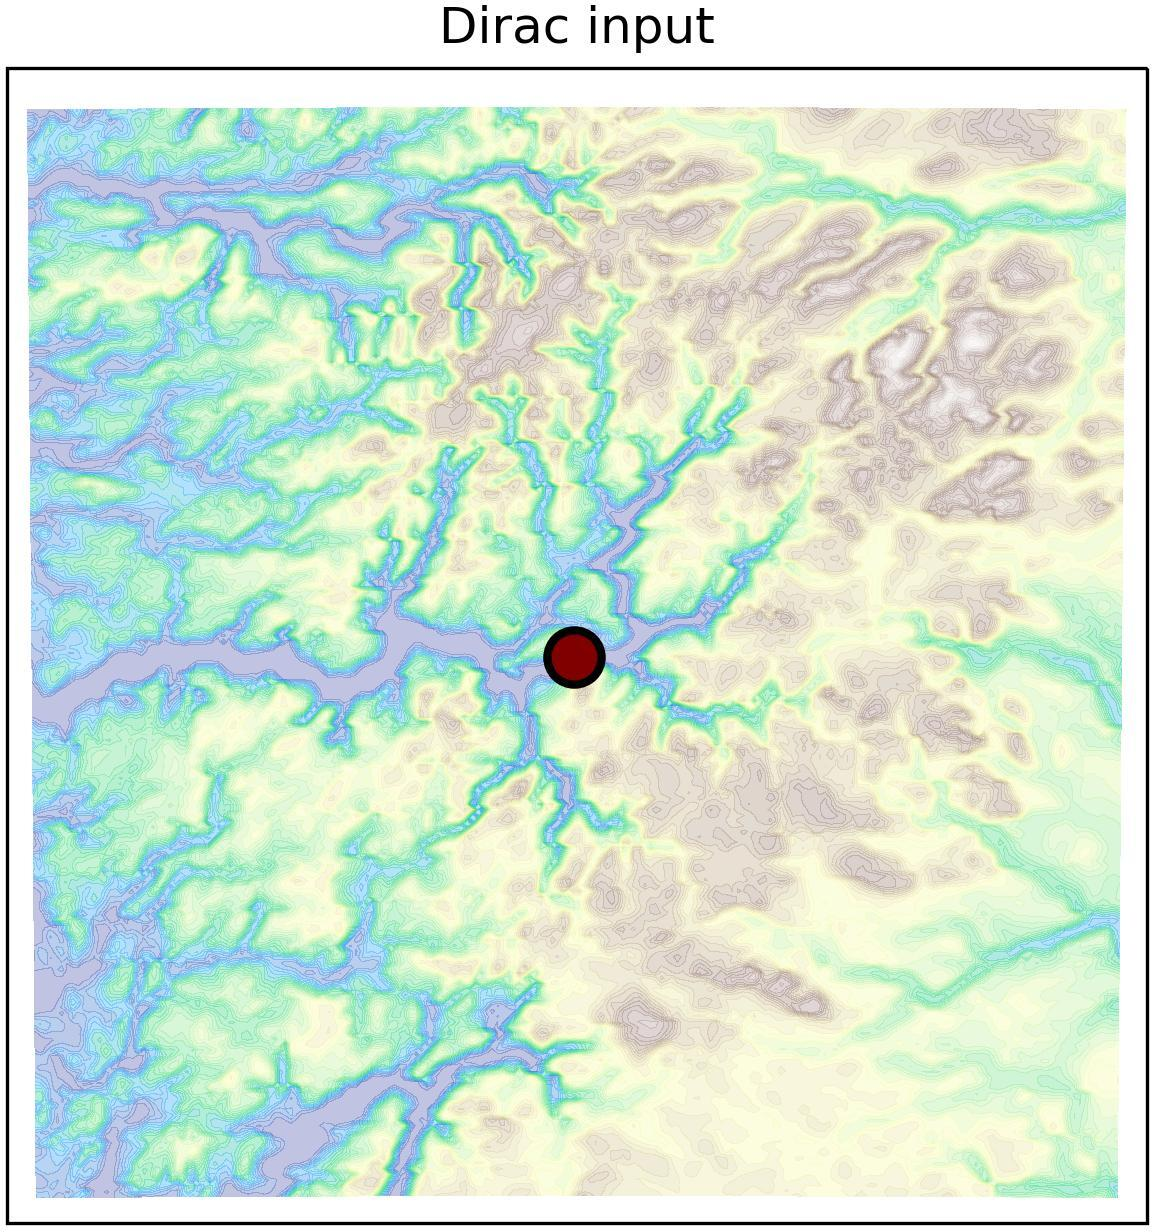
\includegraphics[width=0.33\textwidth]{bottom_1-dirac_input.jpg}
\caption{Dirac test: $\boldsymbol{\delta}^j$} \label{fig:bottom_1-dirac_input}
\end{figure}

\begin{figure}[h!]
\centering
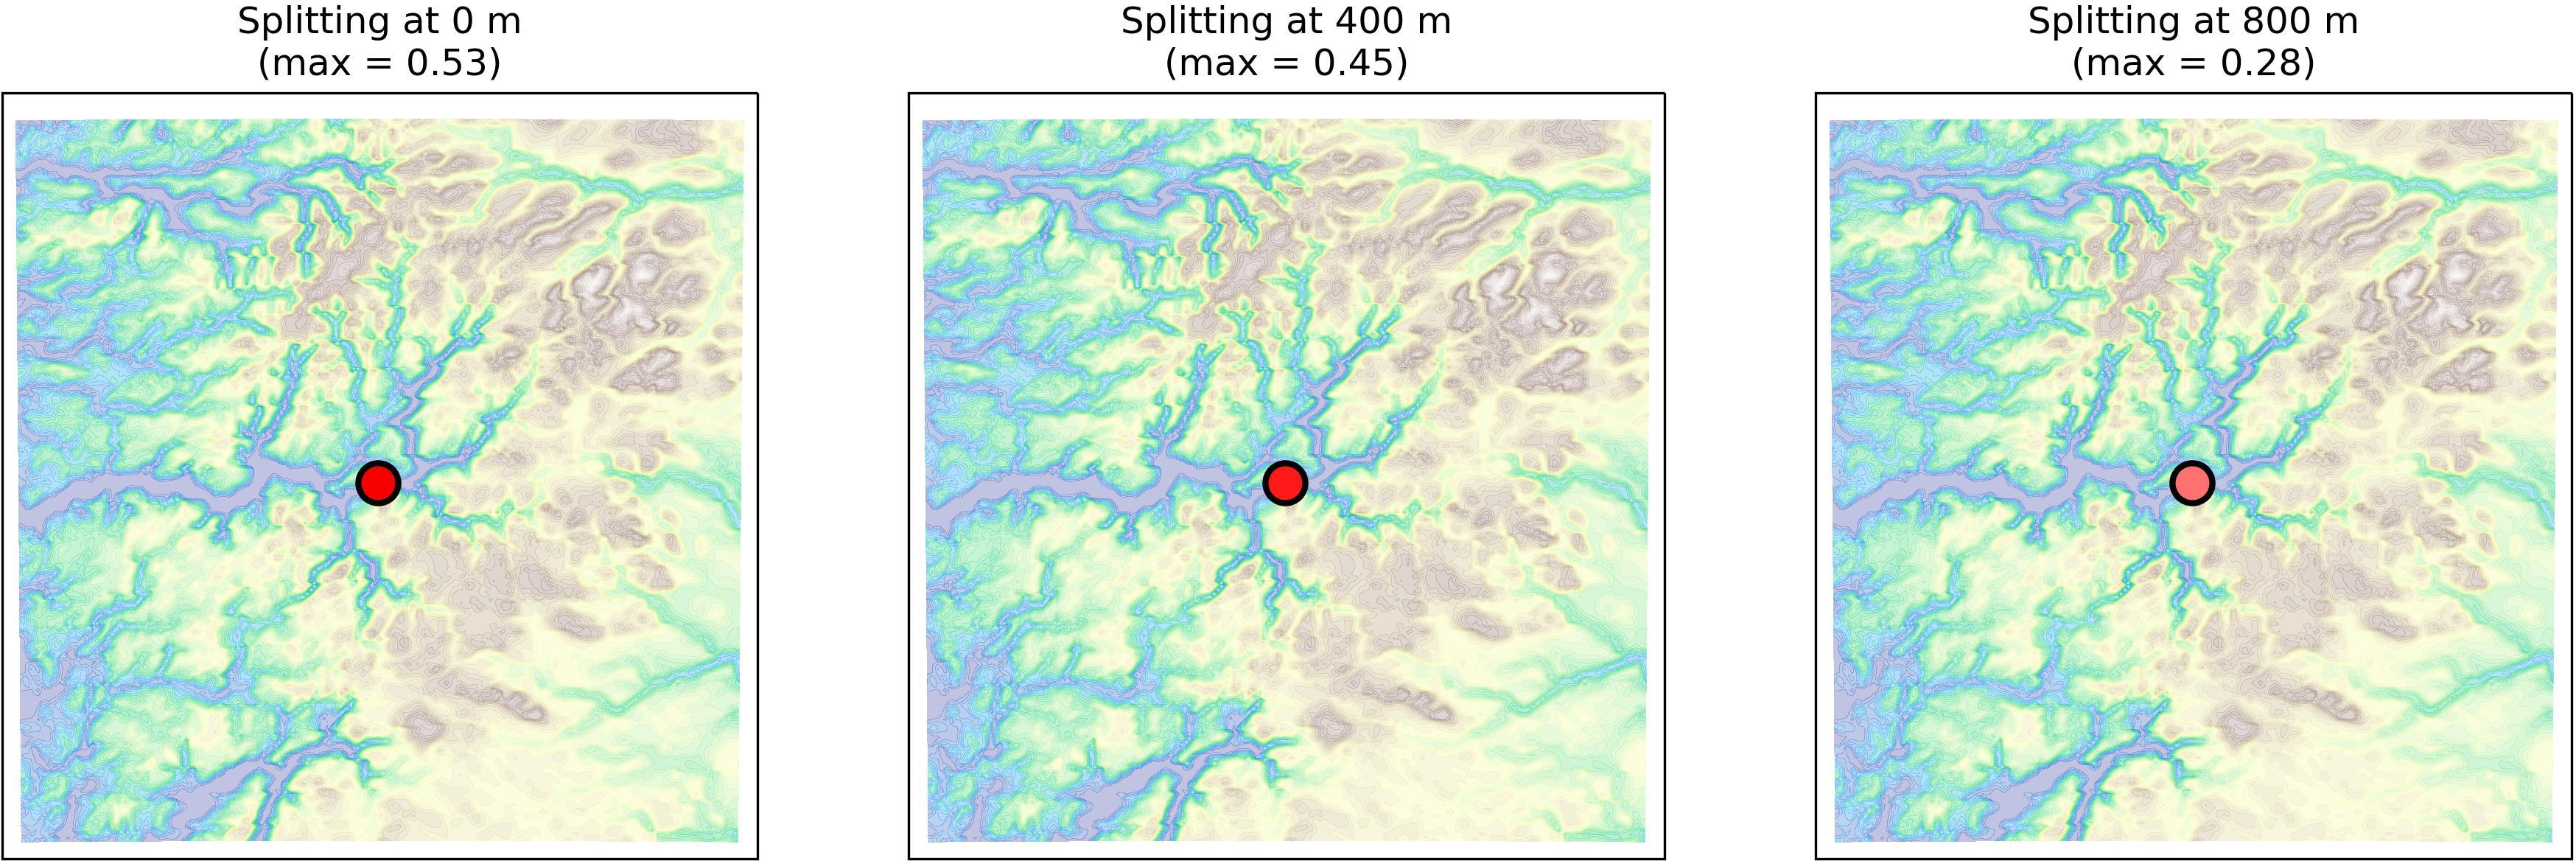
\includegraphics[width=\textwidth]{bottom_2-split.jpg}
\caption{Dirac test: $\mathbf{F}^\text{T} \boldsymbol{\delta}^j$} \label{fig:bottom_2-split}
\end{figure}

\begin{figure}[h!]
\centering
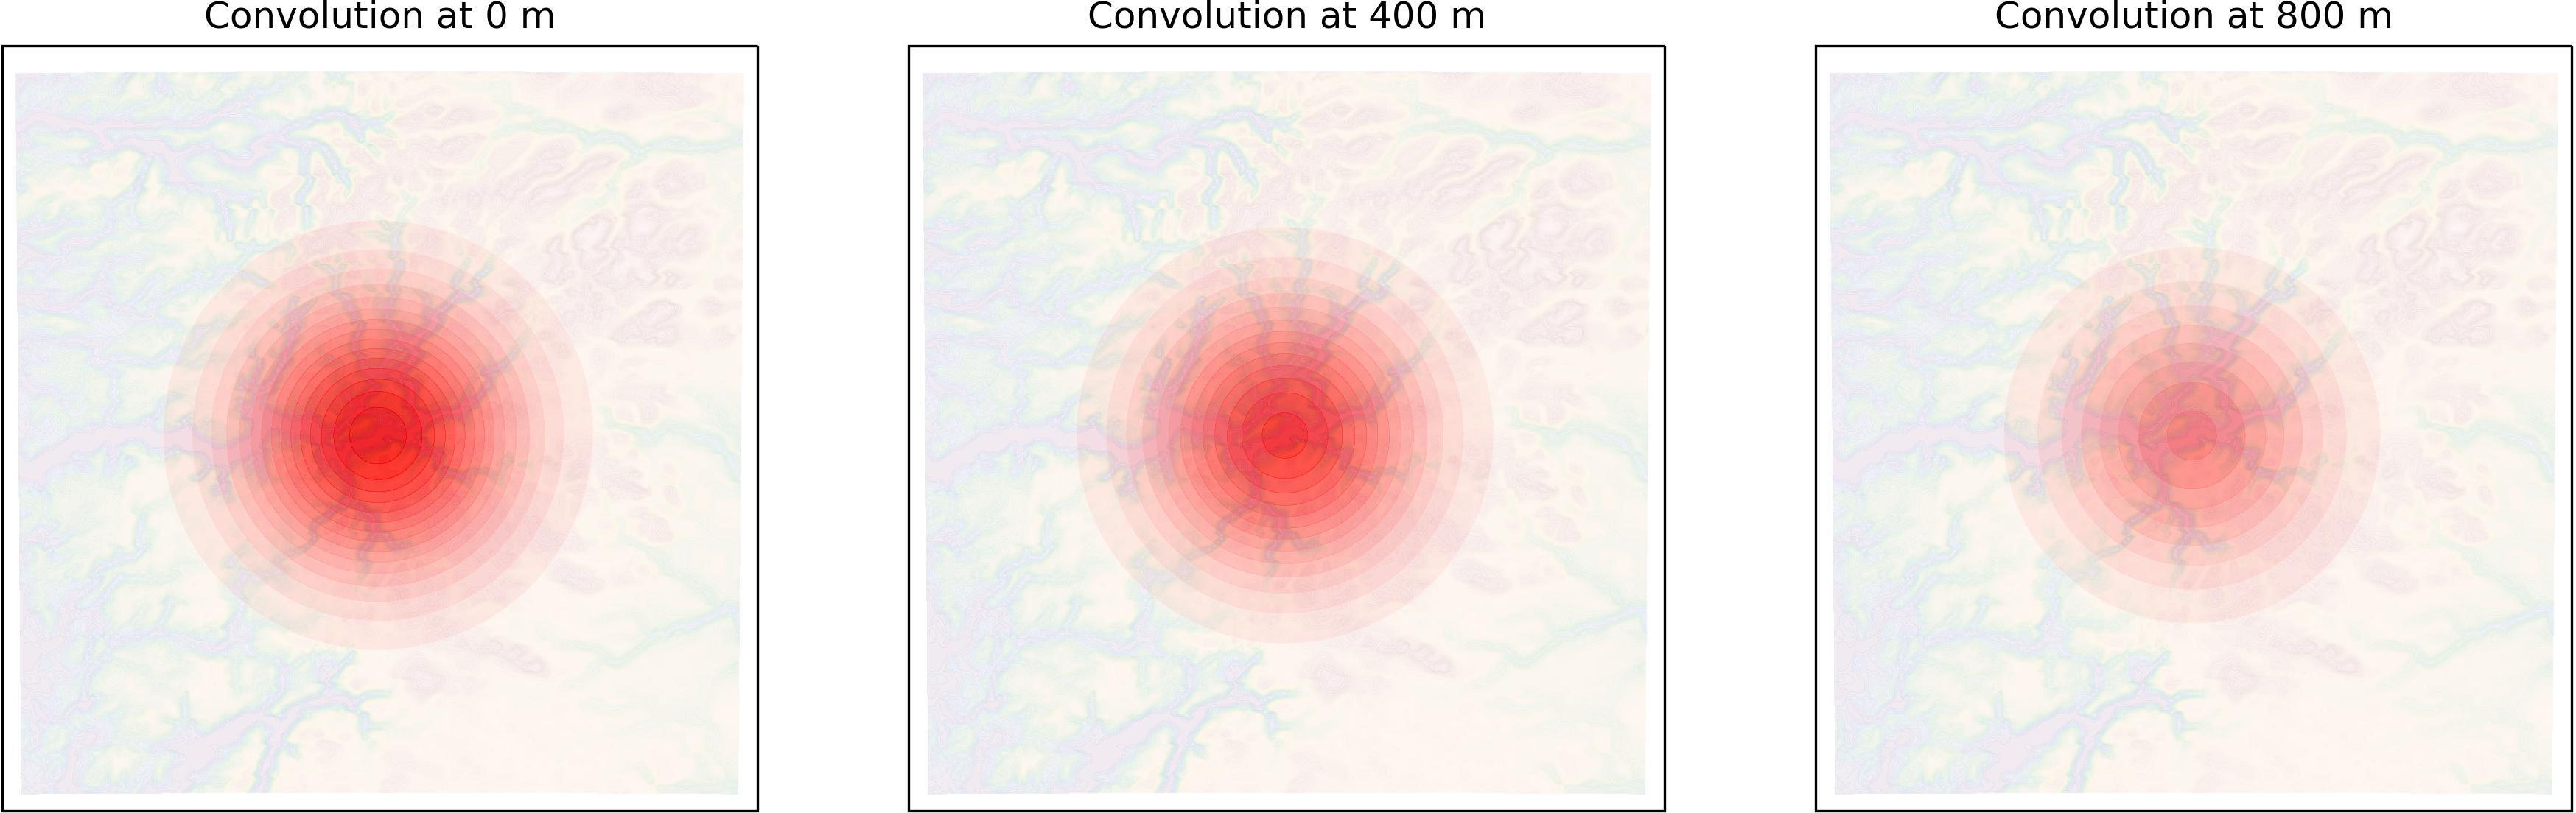
\includegraphics[width=\textwidth]{bottom_3-convolution.jpg}
\caption{Dirac test: $\mathbf{C}_{3D} \mathbf{F}^\text{T} \boldsymbol{\delta}^j$} \label{fig:bottom_3-convolution}
\end{figure}

\begin{figure}[h!]
\centering
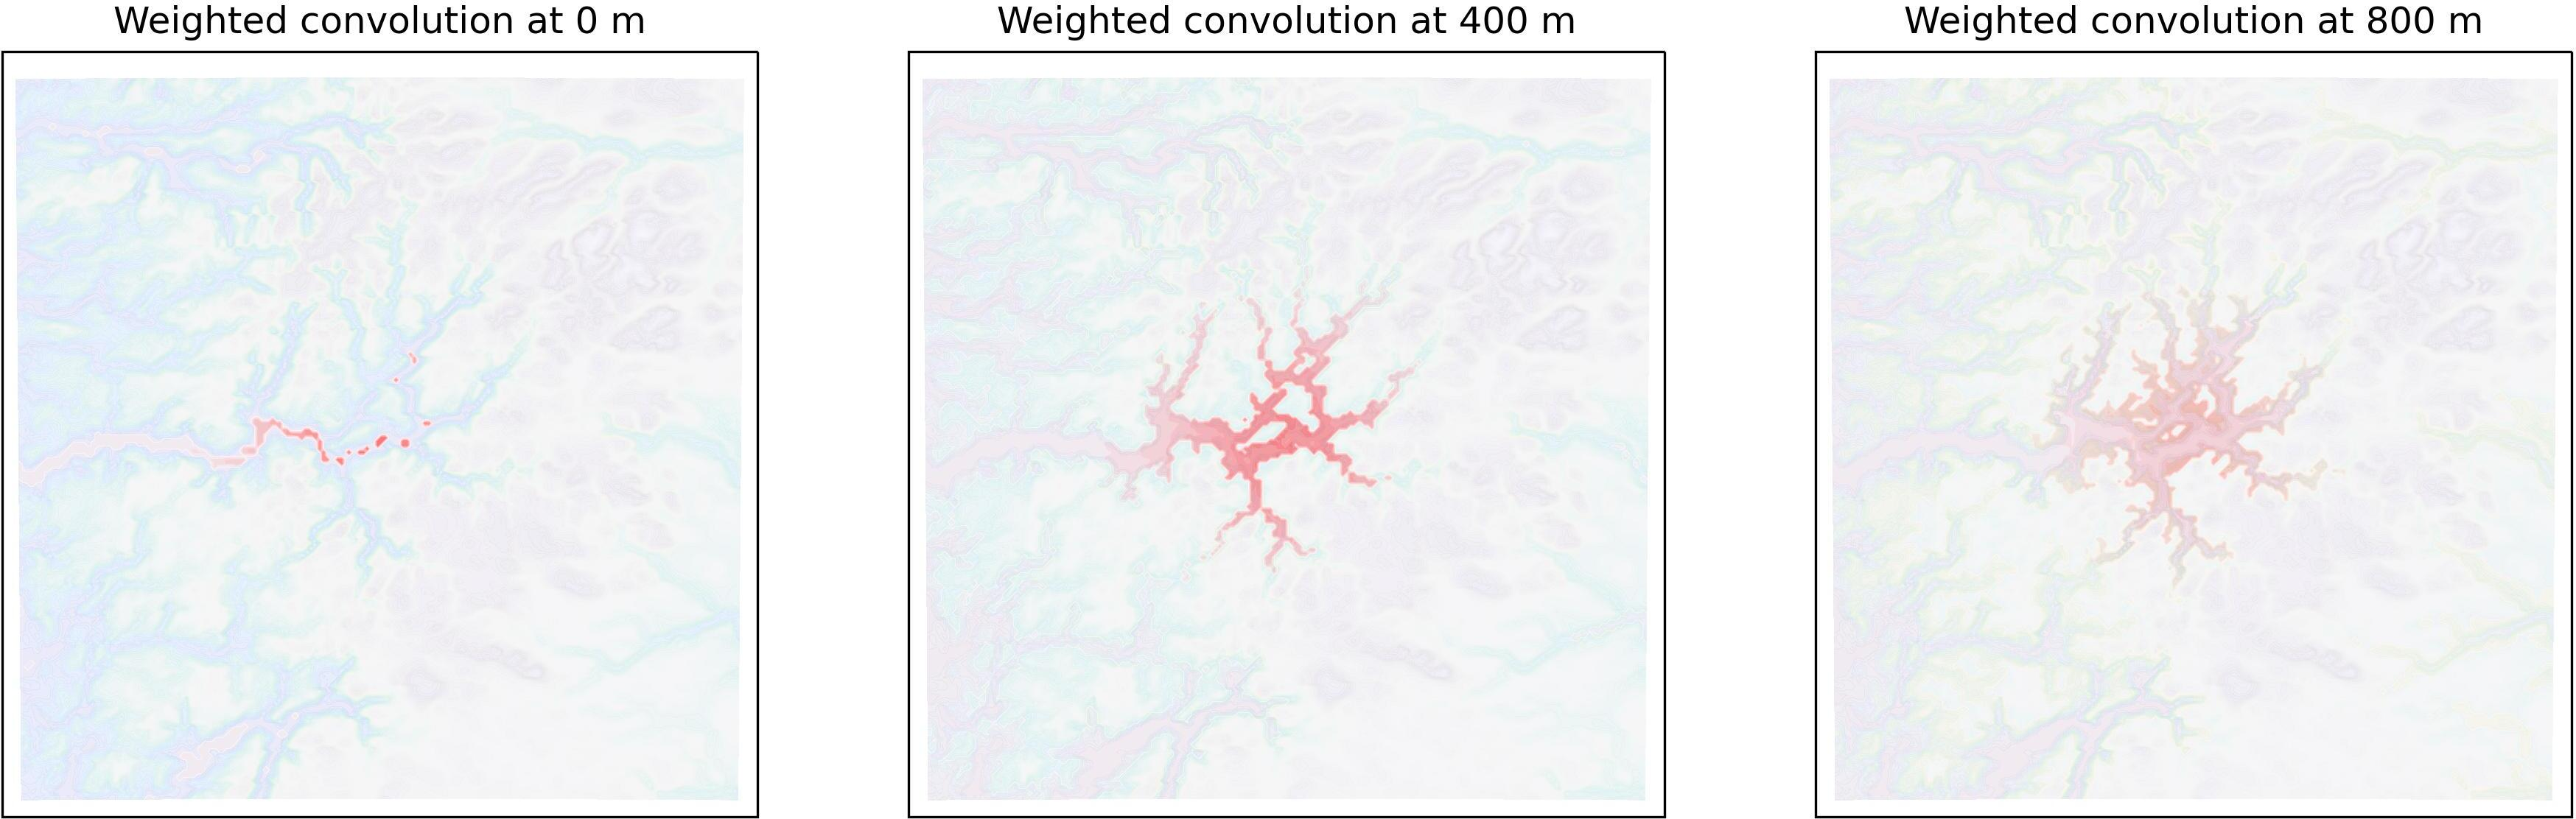
\includegraphics[width=\textwidth]{bottom_4-weighted_convolution.jpg}
\caption{Dirac test: $\mathbf{W} \mathbf{C}_{3D} \mathbf{F}^\text{T} \boldsymbol{\delta}^j$} \label{fig:bottom_4-weighted_convolution}
\end{figure}

\begin{figure}[h!]
\centering
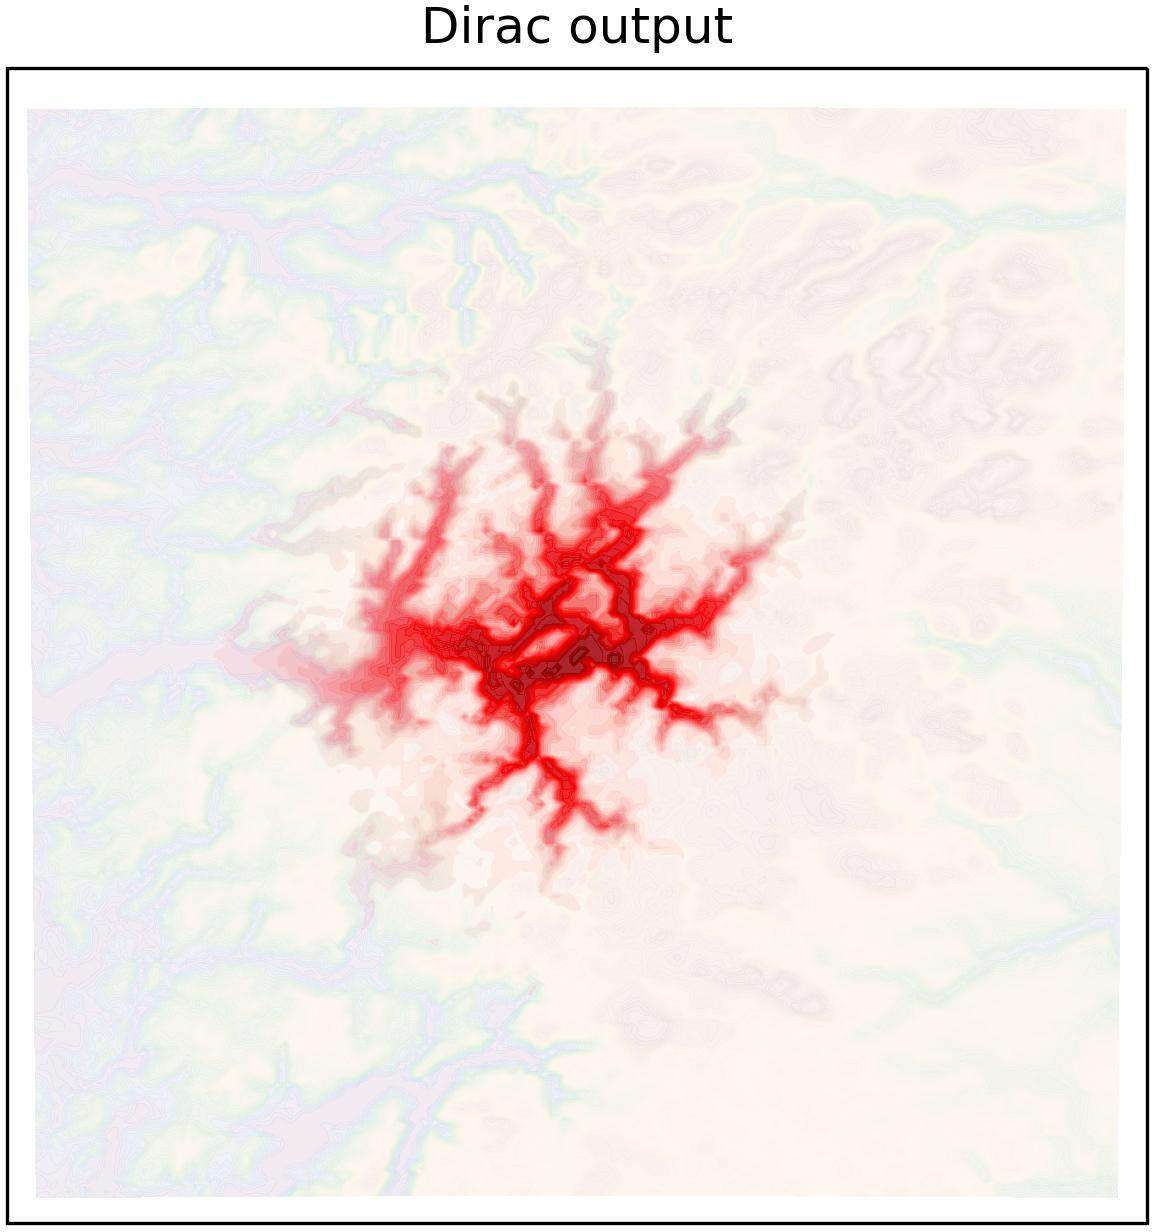
\includegraphics[width=0.33\textwidth]{bottom_5-dirac_output.jpg}
\caption{Dirac test: $\mathbf{F} \mathbf{C}_{3D} \mathbf{F}^\text{T} \boldsymbol{\delta}^j$} \label{fig:bottom_5-dirac_output}
\end{figure}

\begin{figure}[h!]
\centering
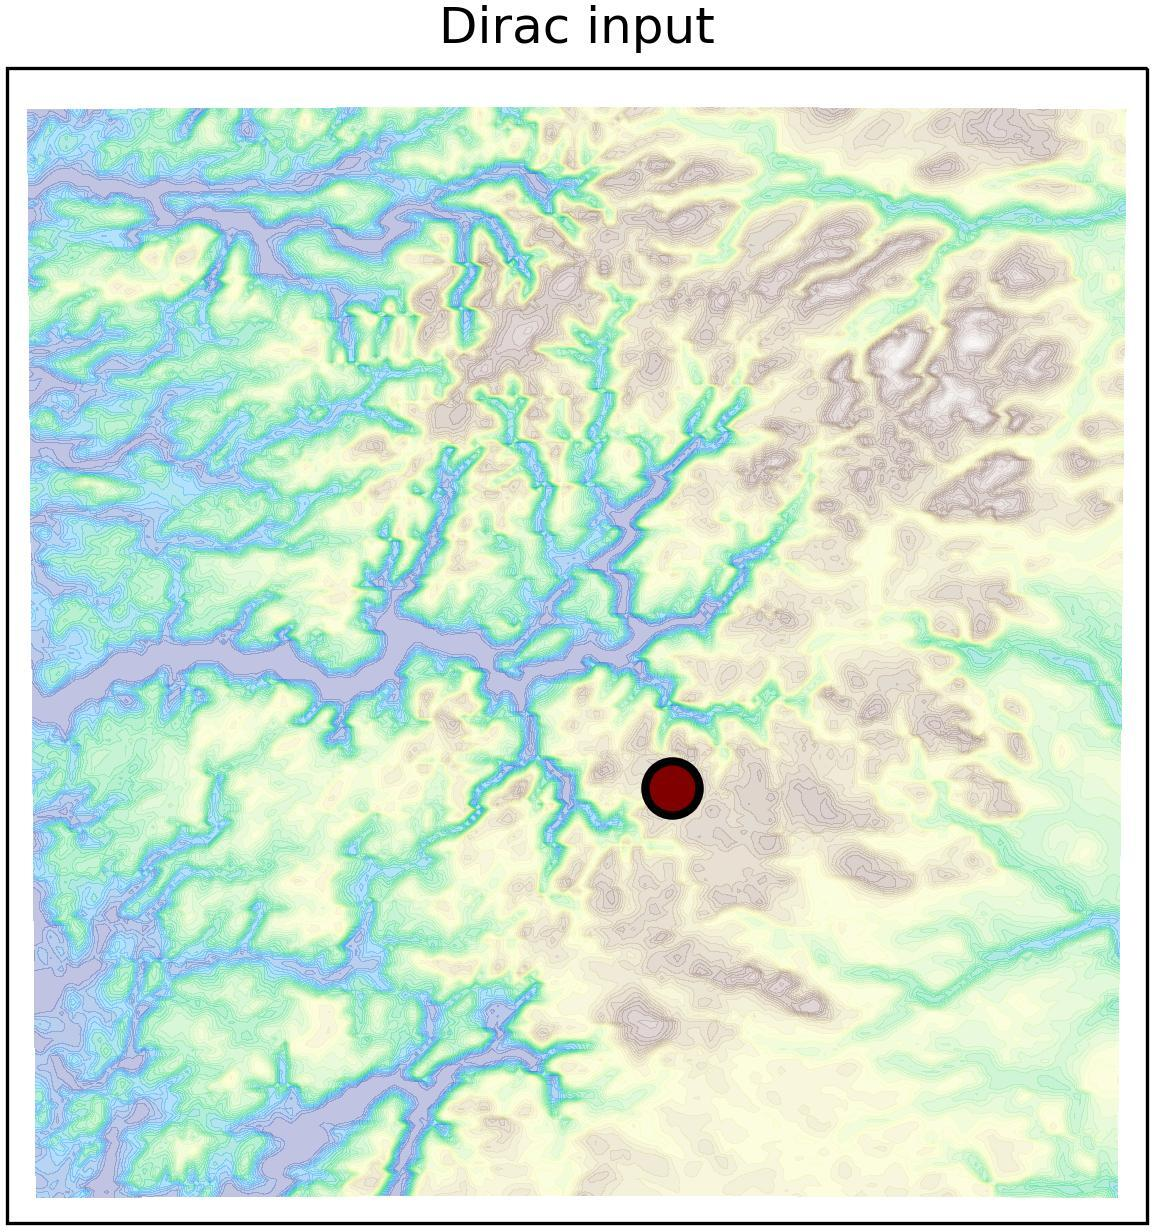
\includegraphics[width=0.33\textwidth]{top_1-dirac_input.jpg}
\caption{Dirac test: $\boldsymbol{\delta}^j$} \label{fig:top_1-dirac_input}
\end{figure}

\begin{figure}[h!]
\centering
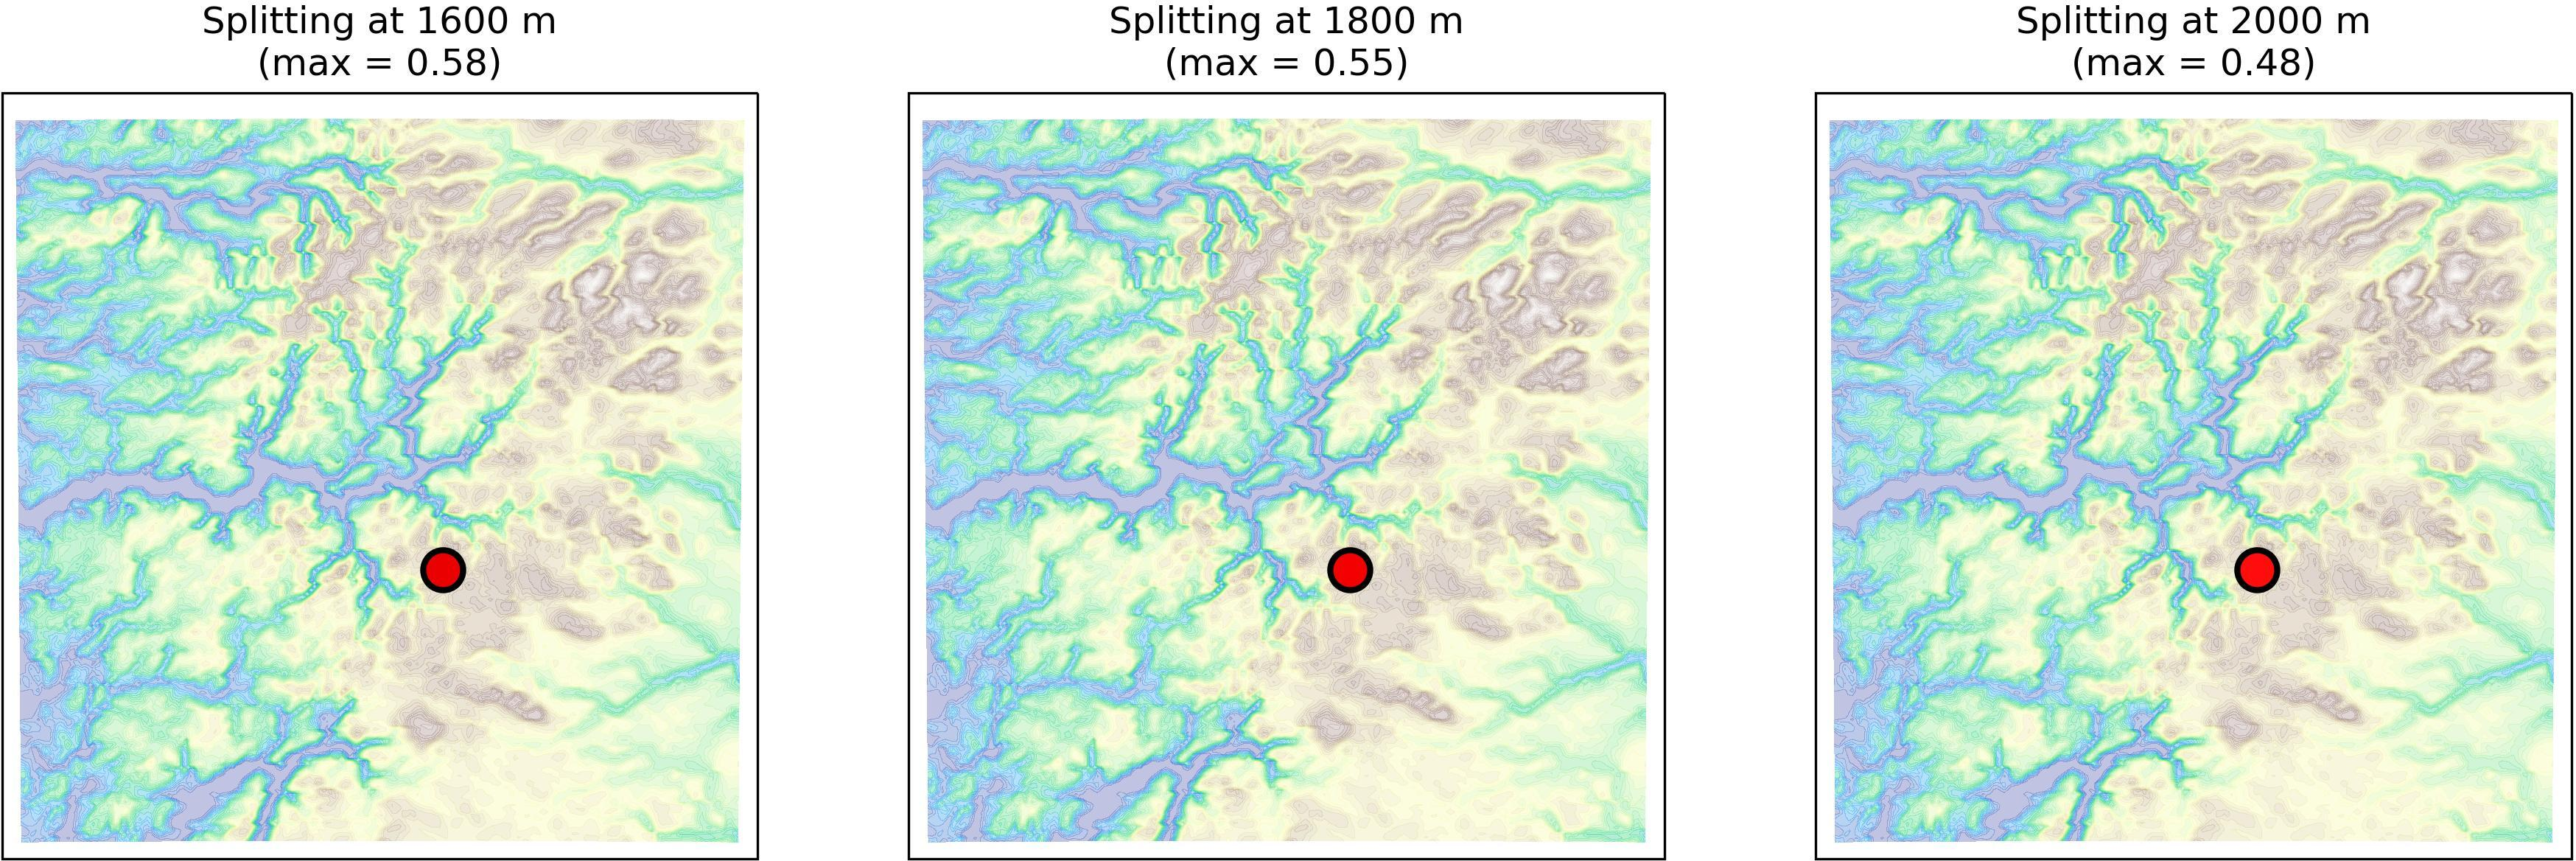
\includegraphics[width=\textwidth]{top_2-split.jpg}
\caption{Dirac test: $\mathbf{F}^\text{T} \boldsymbol{\delta}^j$} \label{fig:top_2-split}
\end{figure}

\begin{figure}[h!]
\centering
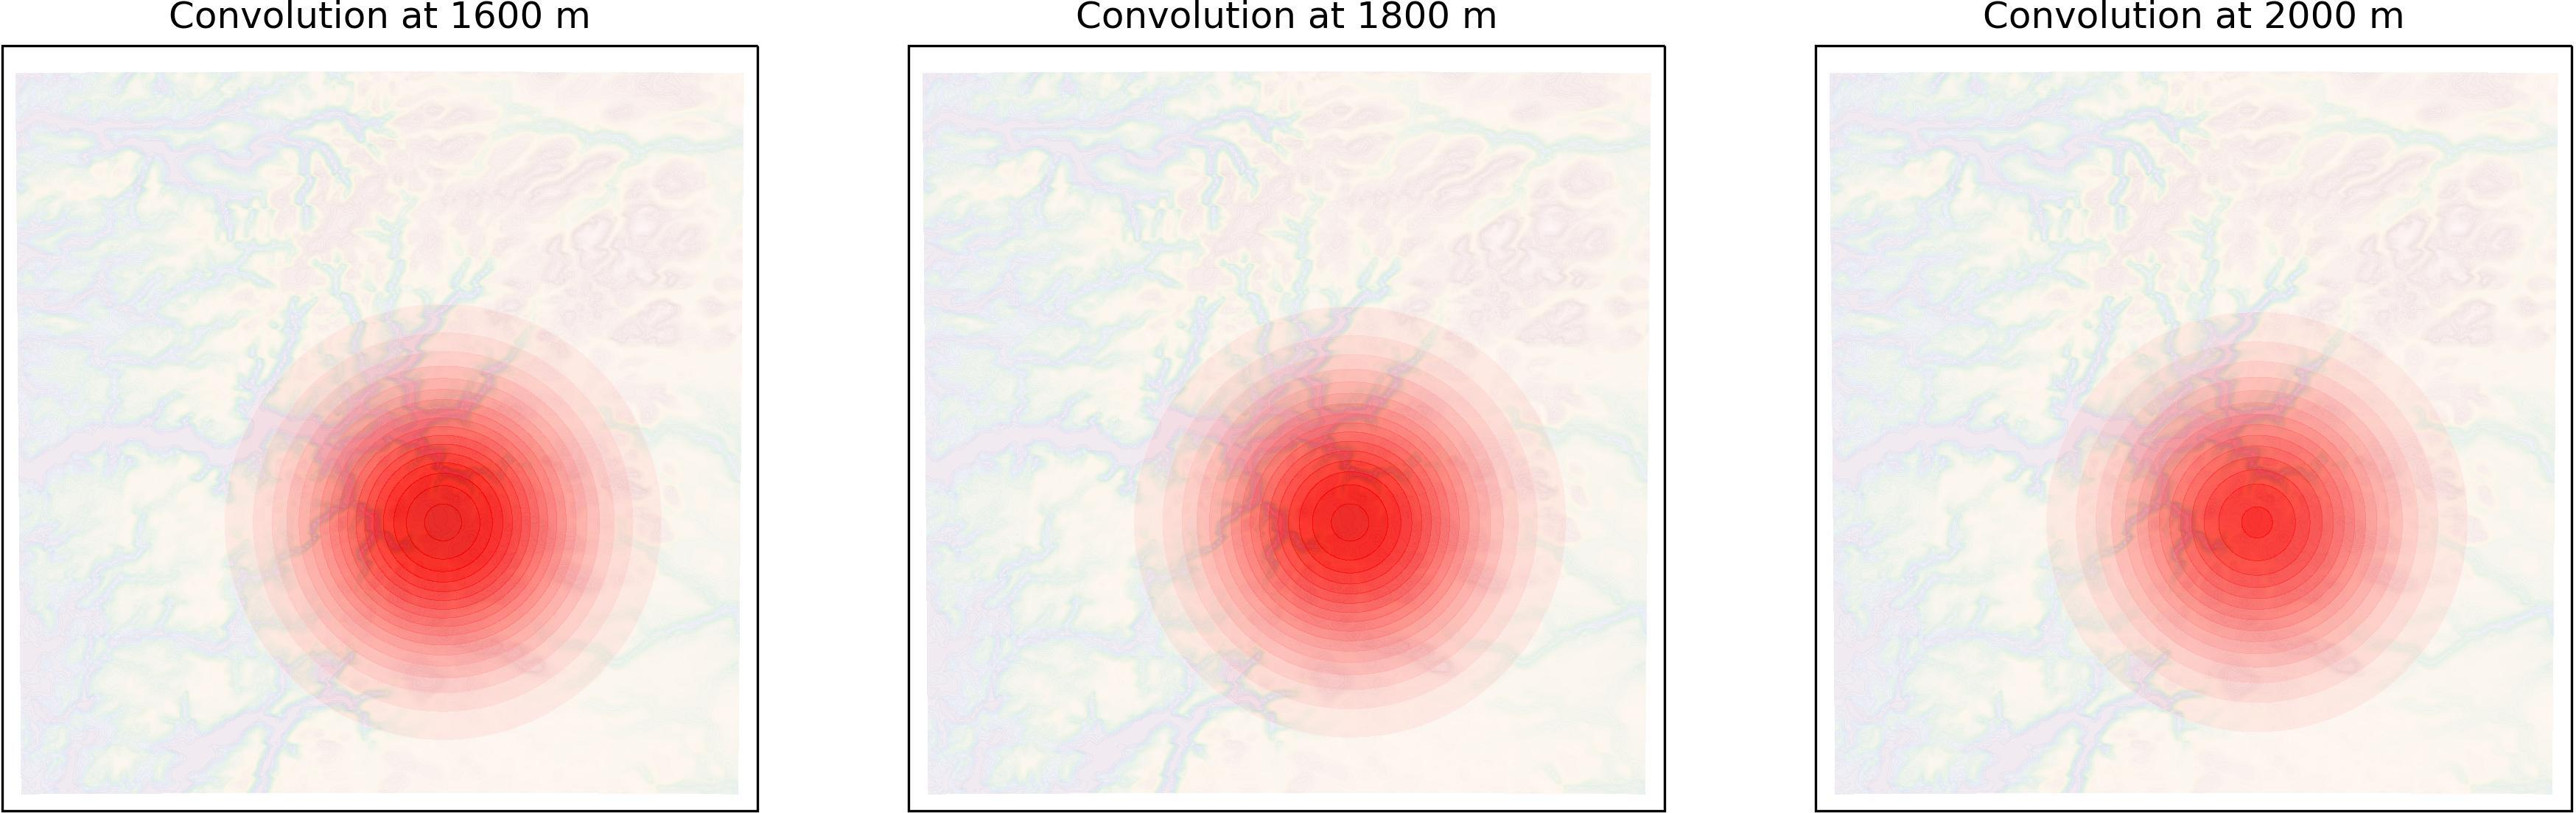
\includegraphics[width=\textwidth]{top_3-convolution.jpg}
\caption{Dirac test: $\mathbf{C}_{3D} \mathbf{F}^\text{T} \boldsymbol{\delta}^j$} \label{fig:top_3-convolution}
\end{figure}

\begin{figure}[h!]
\centering
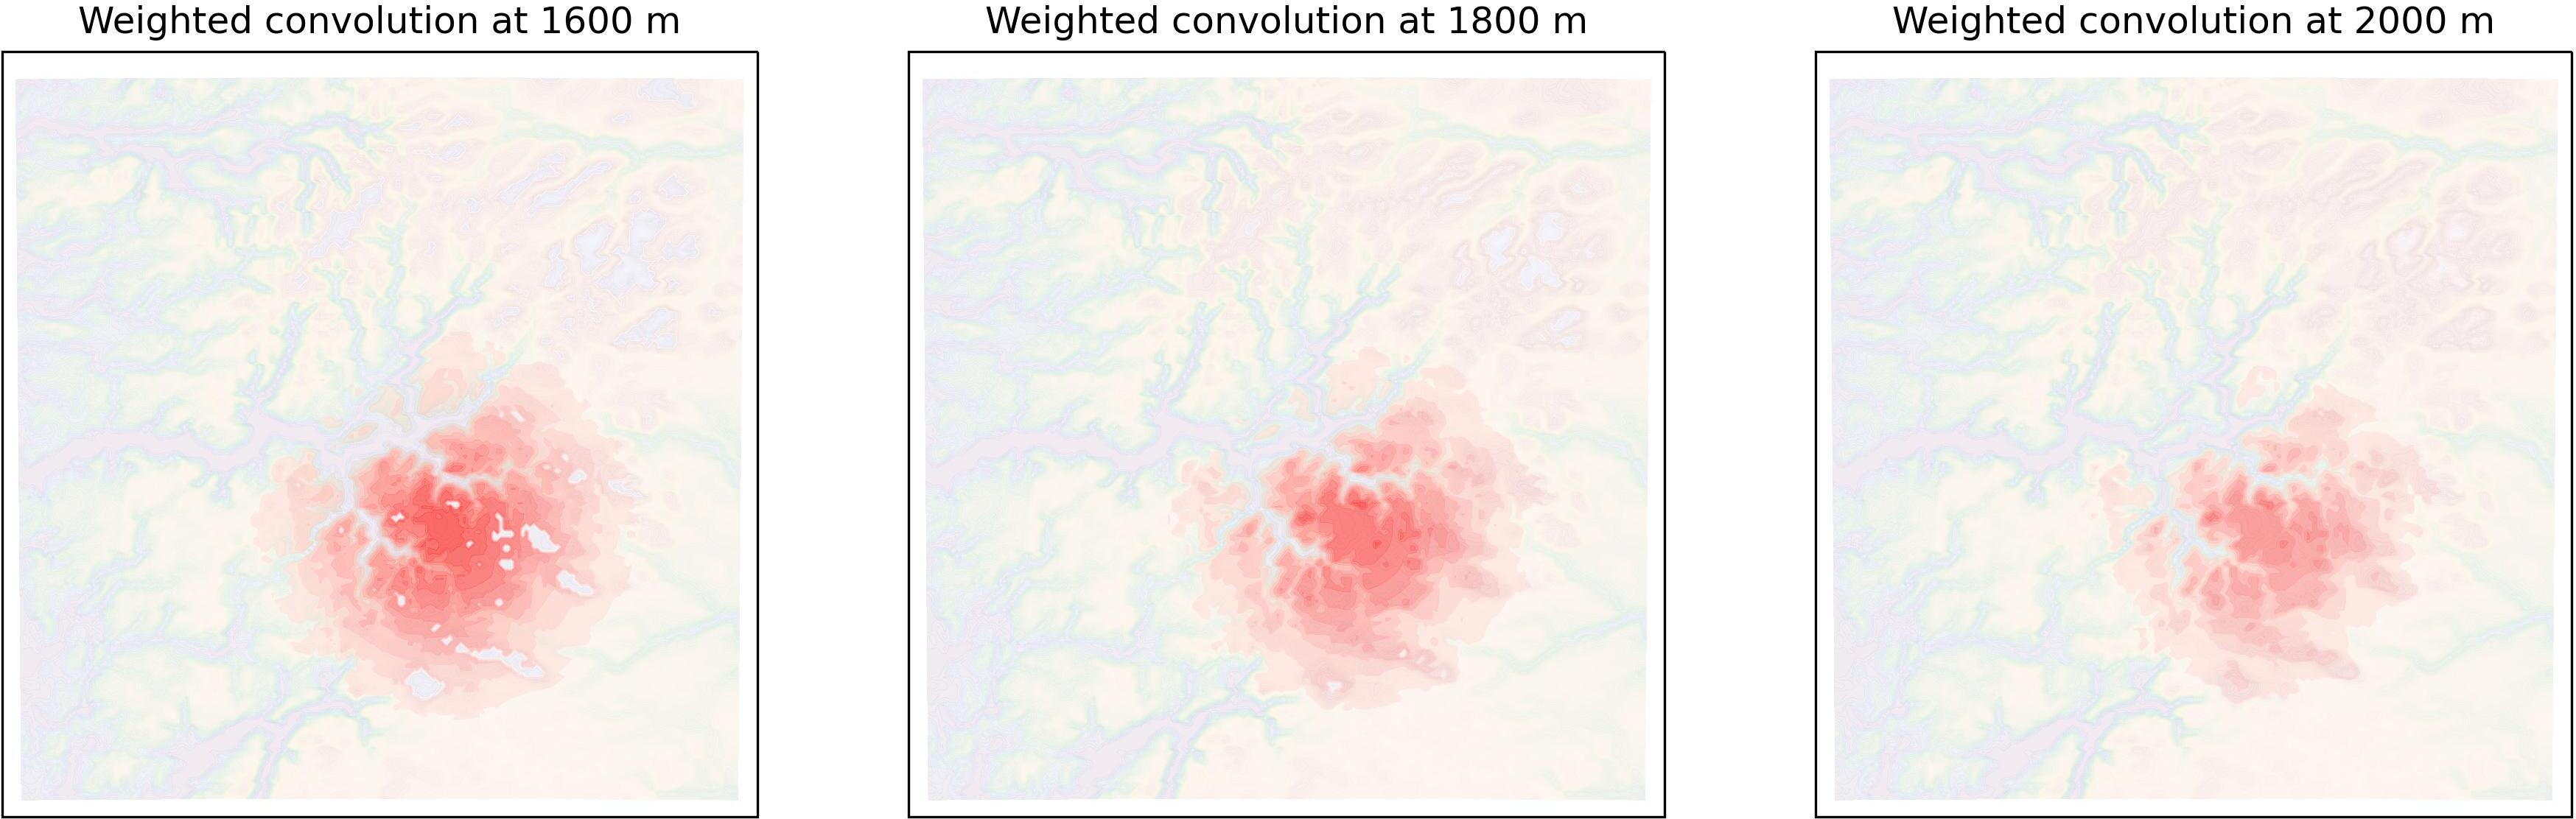
\includegraphics[width=\textwidth]{top_4-weighted_convolution.jpg}
\caption{Dirac test: $\mathbf{W} \mathbf{C}_{3D} \mathbf{F}^\text{T} \boldsymbol{\delta}^j$} \label{fig:top_4-weighted_convolution}
\end{figure}

\begin{figure}[h!]
\centering
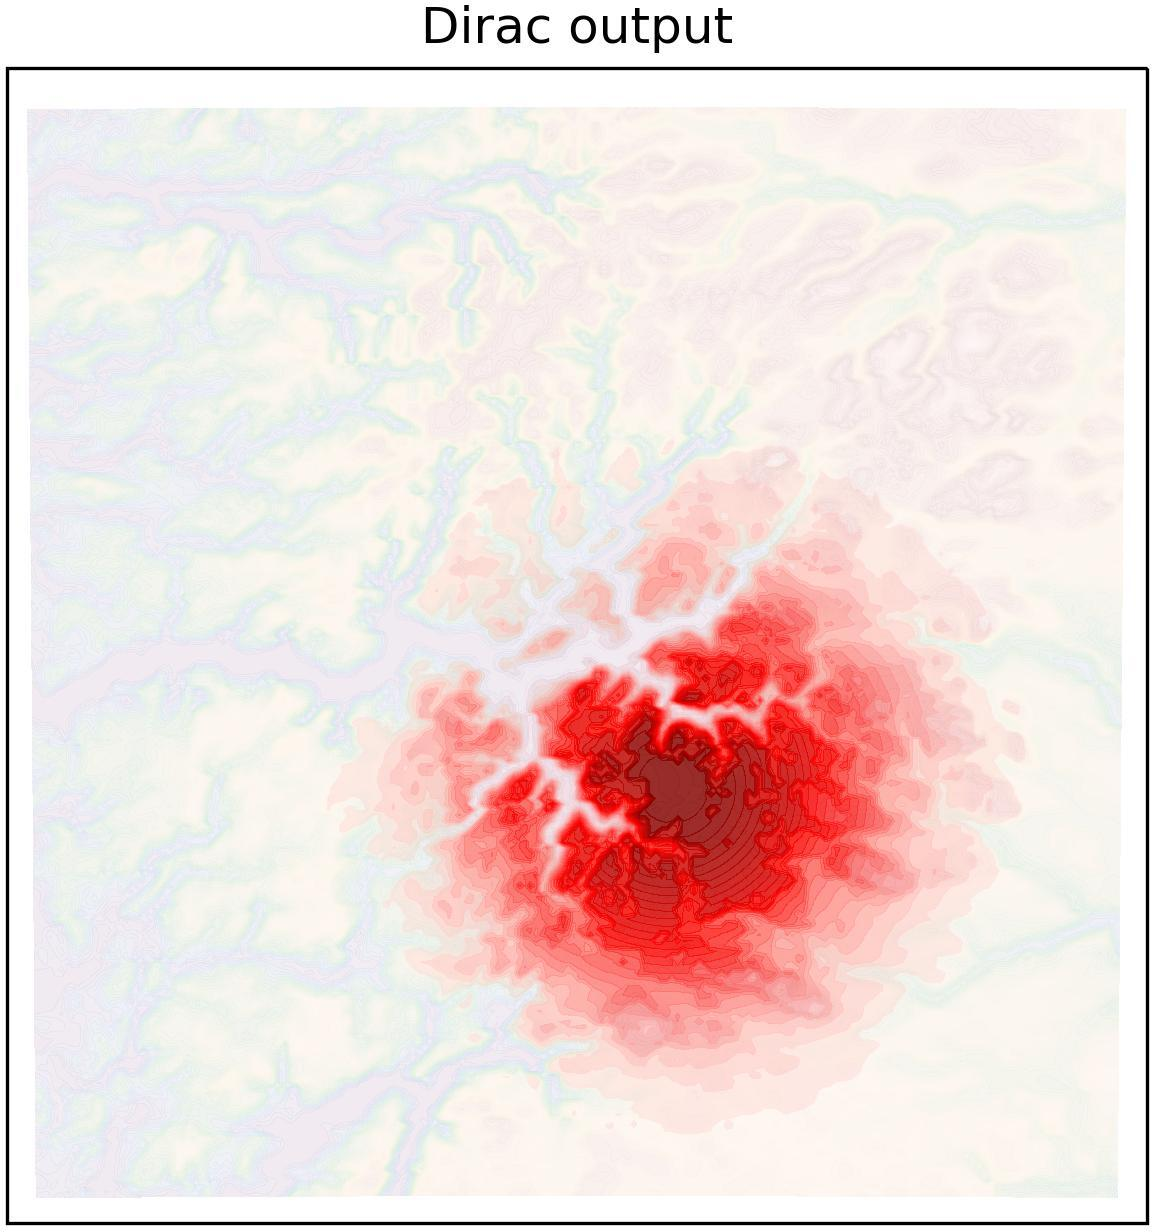
\includegraphics[width=0.33\textwidth]{top_5-dirac_output.jpg}
\caption{Dirac test: $\mathbf{F} \mathbf{C}_{3D} \mathbf{F}^\text{T} \boldsymbol{\delta}^j$} \label{fig:top_5-dirac_output}
\end{figure}

\begin{figure}[h!]
\centering
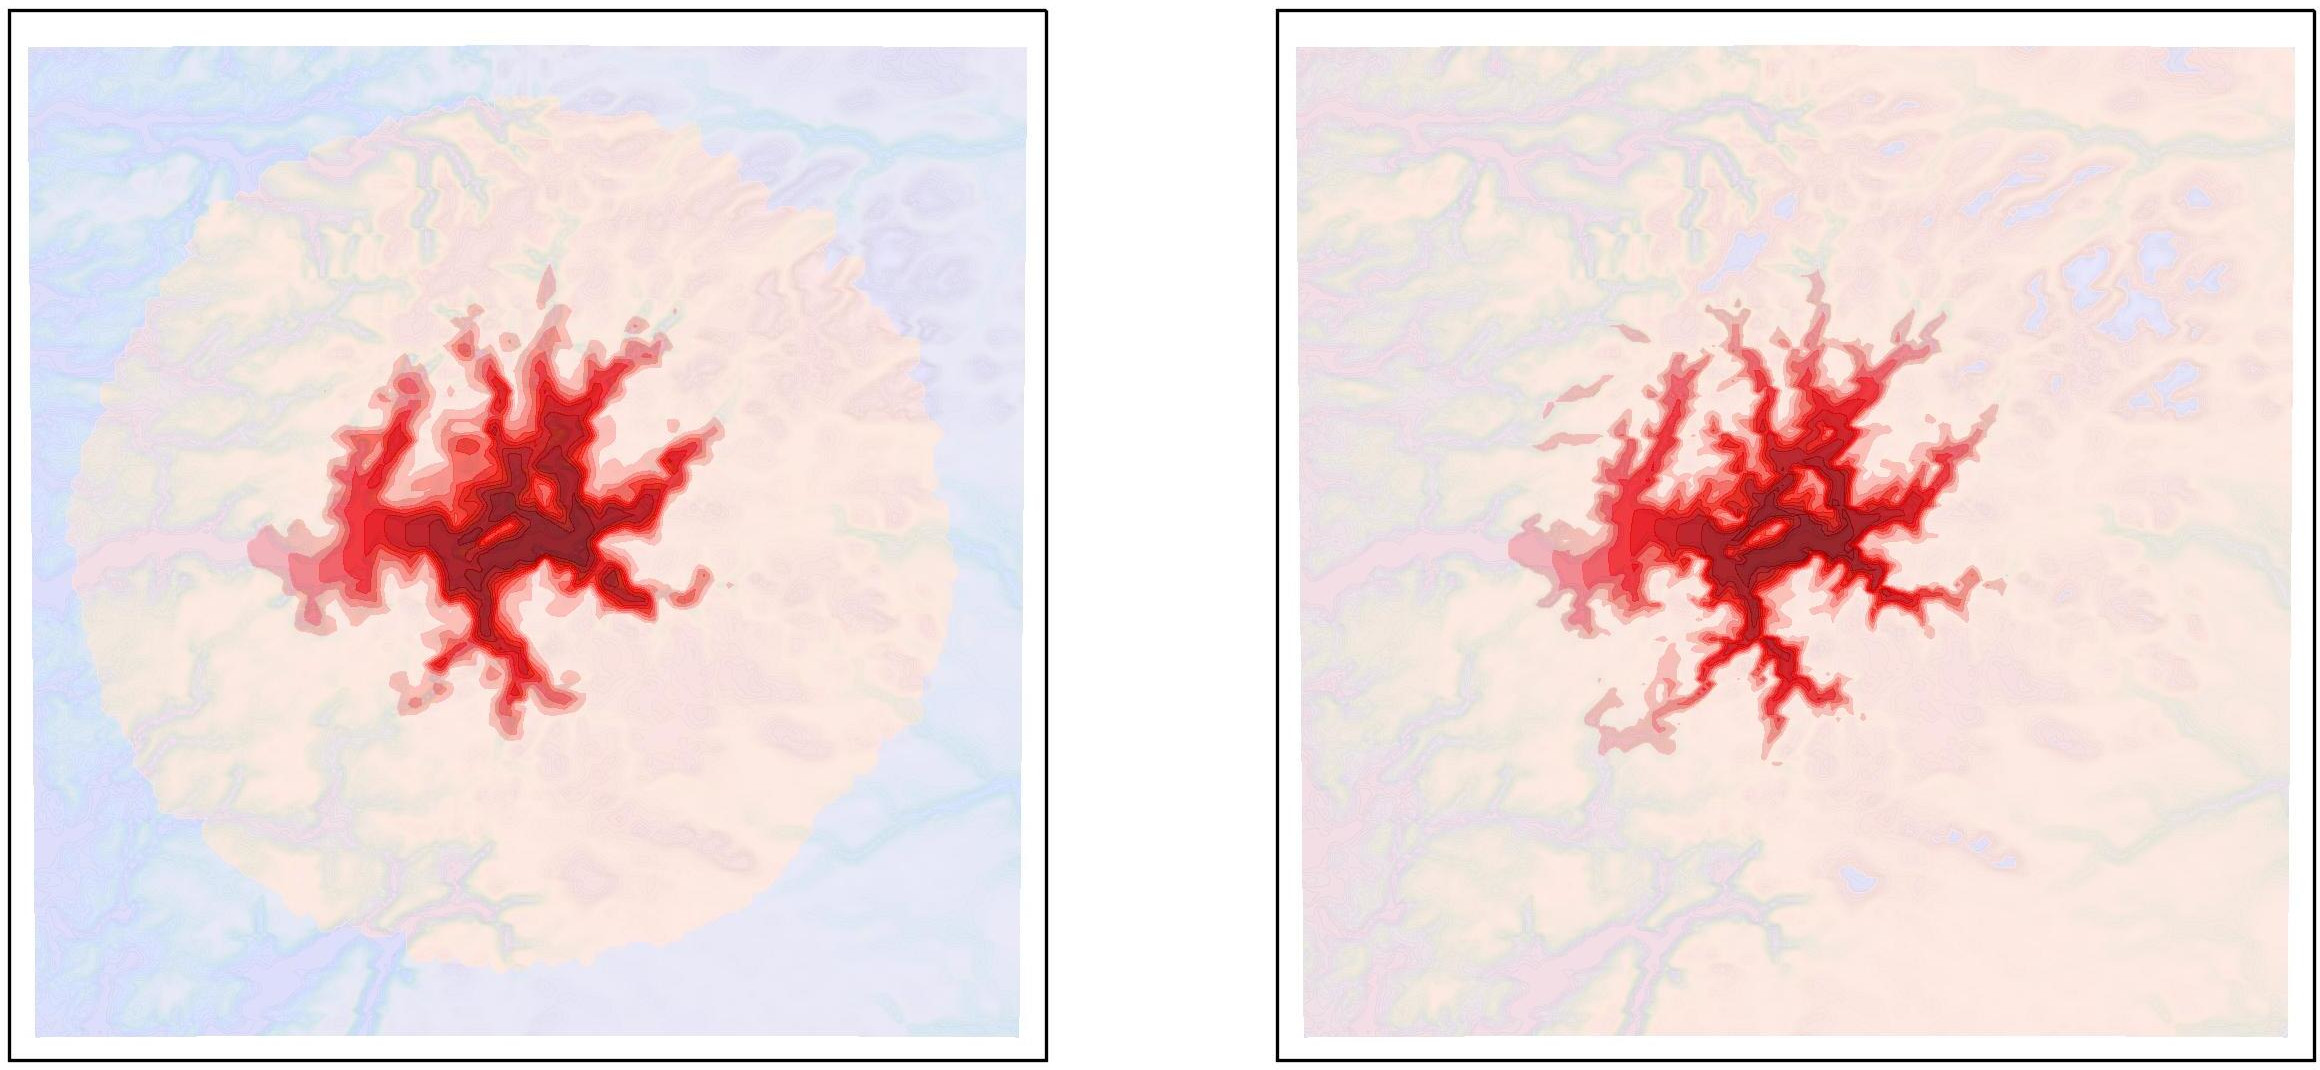
\includegraphics[width=\textwidth]{small.jpg}
\caption{Left: full 3D convolution; right: 2D convolution using shadow levels} \label{fig:small}
\end{figure}

\end{document}
